% ch04-exists-vs-forall.tex — Existential vs Universal Restriction
% Side-by-side comparison of ∃R.C and ∀R.C with domain elements.
% Pedagogical purpose: show that absence in RDF data ≠ absence in interpretation.
\documentclass[tikz,border=5pt]{standalone}
\usepackage{fontspec}
\setmainfont{Times New Roman}
\usepackage{unicode-math}
\setmathfont{Cambria Math}
\usetikzlibrary{shapes.geometric,positioning,fit,backgrounds,arrows.meta}

\begin{document}
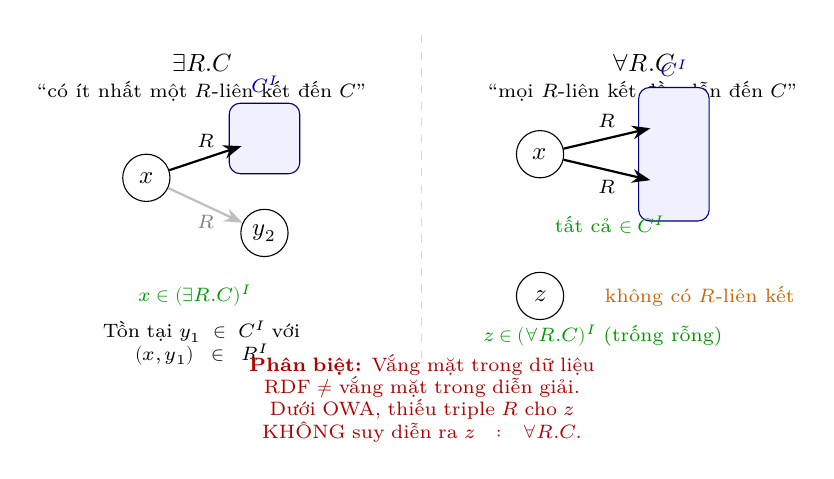
\begin{tikzpicture}[
  elem/.style={circle,draw,minimum size=0.6cm,inner sep=1pt,font=\small},
  classbox/.style={rounded corners=4pt,draw,inner sep=4pt},
  arr/.style={->,>=Stealth,thick},
  note/.style={font=\scriptsize,align=center,text width=3.8cm},
  title/.style={font=\small\bfseries,anchor=north},
]

% === LEFT: ∃R.C ===
\node[title] at (-2.8,3.2) {$\exists R.C$};
\node[font=\scriptsize,anchor=north] at (-2.8,2.85)
  {``có ít nhất một $R$-liên kết đến $C$''};

% Elements
\node[elem] (ex_x) at (-3.5,1.5) {$x$};
\node[elem,fill=blue!10] (ex_y1) at (-2.0,2.0) {$y_1$};
\node[elem] (ex_y2) at (-2.0,0.8) {$y_2$};

% C class region
\node[classbox,fill=blue!6,draw=blue!50!black,fit=(ex_y1),
      label={[font=\scriptsize,text=blue!70!black]north:$C^I$}] {};

% R arrows
\draw[arr] (ex_x) -- node[midway,above,font=\scriptsize]{$R$} (ex_y1);
\draw[arr,gray!50] (ex_x) -- node[midway,below,font=\scriptsize,gray]{$R$} (ex_y2);

% Check mark
\node[font=\scriptsize,text=green!60!black] at (-2.8,0.0)
  {$x \in (\exists R.C)^I$ ✓};
\node[note] at (-2.8,-0.6)
  {Tồn tại $y_1 \in C^I$ với\\$(x,y_1) \in R^I$};

% Divider
\draw[gray!30,dashed] (0,-0.8) -- (0,3.4);

% === RIGHT: ∀R.C ===
\node[title] at (2.8,3.2) {$\forall R.C$};
\node[font=\scriptsize,anchor=north] at (2.8,2.85)
  {``mọi $R$-liên kết đều dẫn đến $C$''};

% Case 1: has successors, all in C
\node[elem] (un_x) at (1.5,1.8) {$x$};
\node[elem,fill=blue!10] (un_y1) at (3.2,2.2) {$y_1$};
\node[elem,fill=blue!10] (un_y2) at (3.2,1.4) {$y_2$};

\node[classbox,fill=blue!6,draw=blue!50!black,fit=(un_y1)(un_y2),
      label={[font=\scriptsize,text=blue!70!black]north:$C^I$}] {};

\draw[arr] (un_x) -- node[midway,above,font=\scriptsize]{$R$} (un_y1);
\draw[arr] (un_x) -- node[midway,below,font=\scriptsize]{$R$} (un_y2);

\node[font=\scriptsize,text=green!60!black] at (2.3,0.9) {✓ tất cả $\in C^I$};

% Case 2: no successors (vacuously true)
\node[elem] (vac_x) at (1.5,0.0) {$z$};
\node[font=\scriptsize,text=orange!80!black,anchor=west] at (2.2,0.0)
  {không có $R$-liên kết};
\node[font=\scriptsize,text=green!60!black] at (2.3,-0.5)
  {$z \in (\forall R.C)^I$ (trống rỗng)};

% Bottom warning
\node[font=\scriptsize,text=red!70!black,align=center,text width=7cm]
  at (0,-1.3)
  {\textbf{Phân biệt:} Vắng mặt trong dữ liệu RDF $\neq$ vắng mặt trong diễn giải.\\
   Dưới OWA, thiếu triple $R$ cho $z$ KHÔNG suy diễn ra $z : \forall R.C$.};

\end{tikzpicture}
\end{document}
